\documentclass[a4paper,11pt]{article}

\usepackage[frenchb]{babel}
\usepackage[T1]{fontenc}
\usepackage[utf8]{inputenc}
\usepackage{graphicx}


\begin{document}

\title{Rapport du Projet Web}
\author{Samuel Bricas\\Thibaut Castanié}
\date{28/04/2014}


\maketitle
\vspace{4em}
\tableofcontents

\maketitle

\newpage
\section{Conception}
\subsection{Représentation de la base de donnée, après analyse}
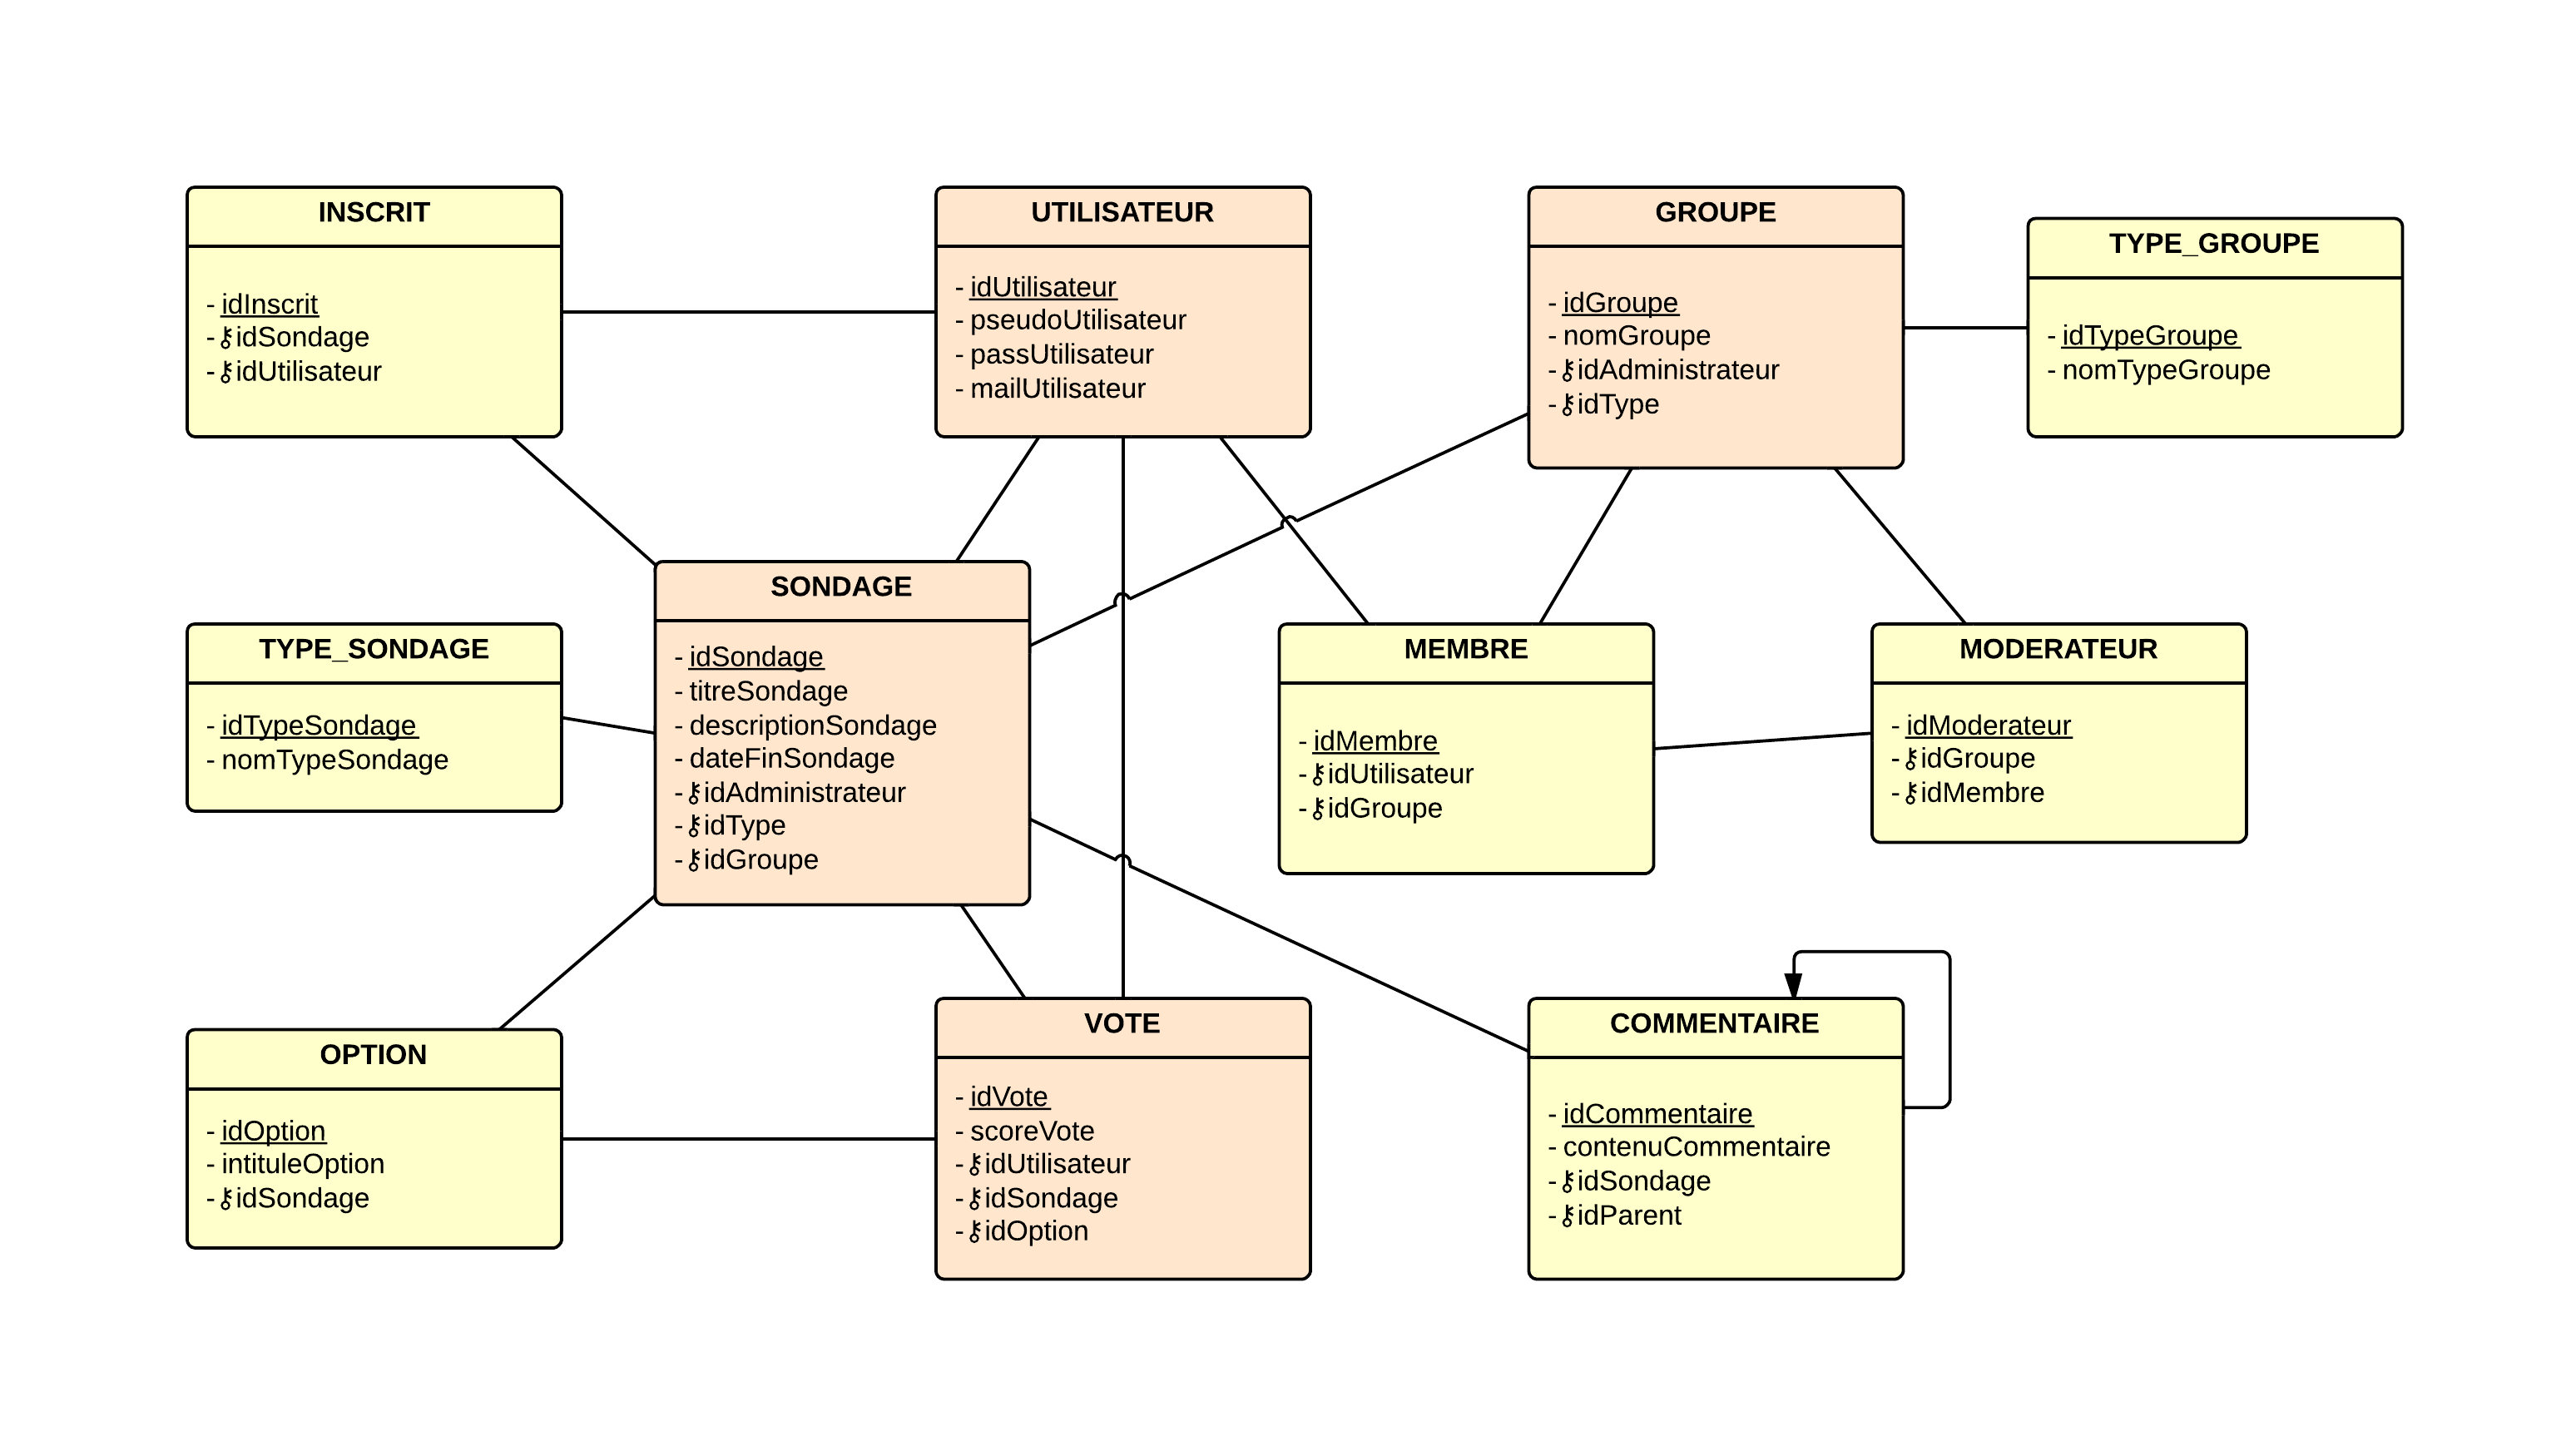
\includegraphics[scale=0.18, angle=90]{BddProjetWeb.png}
\section{Technique utilisée}
\paragraph{}
Dans un premier temps, nous avons analysé avec précision le sujet et nous avons élaboré un premier diagramme de classe rapide au brouillon. Puis nous l'avons peu à peu amélioré pour obtenir le résultat donné dans la partie précédente.
\paragraph{}Nous nous sommes ensuite séparés le travail en deux, afin d'être plus performant. L'un deux nous a créé les modèles de classes utilisés dans le projet ainsi qu'une grande partie des requêtes effectuées sur la base de données, tandis que l'autre s'occupait de réaliser les vues de façon à représenter toutes les information demandées, et de mettre en place l'architecture de type Modèle-Vue-Contrôleur du projet.
\paragraph{}Enfin, nous avons mis notre travail en commun et nous avons travaillé ensemble pour finir le projet. Nous avons mis en relation les modèles avec la vue, par le biais des contrôleurs. Nous nous sommes ainsi occupés de toutes les action telles que la connexion, l'inscription, mais aussi la création de groupes, la visualisation des sondages, etc... Durant cette étape, nous avons dû rajouter de nouvelles requêtes dans les modèles pour répondre à nos besoins.
\section{Outils utilisés}
\paragraph{Lucidchart} Pour créer notre diagramme de classe, nous avons utilisé l'application web \textbf{Lucidchart} (\texttt{www.lucidchart.com/}), qui permet de travailler collaborativement sur des schémas fonctionnels.
\paragraph{Dropbox} Nous avons utilisé le service \textbf{Dropbox} dans le but de pouvoir partager notre projet entre nous. Nous avons créé un dossier partagés entre nos deux comptes, dans lequel nous avons mis l'ensemble des fichiers et répertoires contenant notre projet. A chaque fois que l'un d'entre nous travaillait sur le projet, il mettait à jour le répertoire partagé. Nous n'avons pas utilisé de service plus spécialisé dans ce domaine (tels que svn ou github), car nous avons jugé leur utilisation plutôt inadaptée à notre petit projet et notre petite équipe.
\paragraph{Langages Web} Nous avons utilisé en majeure partie les langages \texttt{HTML} et \texttt{CSS}, ainsi que du \texttt{PHP}. Nous avons utilisé un peu de \texttt{javascript} pour de petites fonctions qui améliorent le confort de l'utilisateur. Notre base de donnée est stockée sur les serveurs de la fac (\textit{venus}) et nous avons fait des requête en \texttt{SQL}. Pour les mettre en relation avec nos modèles \texttt{PHP}, nous avons utilisé l'interface \texttt{PDO}.

\end{document}